% Options for packages loaded elsewhere
\PassOptionsToPackage{unicode}{hyperref}
\PassOptionsToPackage{hyphens}{url}
%
\documentclass[
  11pt,
]{article}
\usepackage{lmodern}
\usepackage{amssymb,amsmath}
\usepackage{ifxetex,ifluatex}
\ifnum 0\ifxetex 1\fi\ifluatex 1\fi=0 % if pdftex
  \usepackage[T1]{fontenc}
  \usepackage[utf8]{inputenc}
  \usepackage{textcomp} % provide euro and other symbols
\else % if luatex or xetex
  \usepackage{unicode-math}
  \defaultfontfeatures{Scale=MatchLowercase}
  \defaultfontfeatures[\rmfamily]{Ligatures=TeX,Scale=1}
\fi
% Use upquote if available, for straight quotes in verbatim environments
\IfFileExists{upquote.sty}{\usepackage{upquote}}{}
\IfFileExists{microtype.sty}{% use microtype if available
  \usepackage[]{microtype}
  \UseMicrotypeSet[protrusion]{basicmath} % disable protrusion for tt fonts
}{}
\makeatletter
\@ifundefined{KOMAClassName}{% if non-KOMA class
  \IfFileExists{parskip.sty}{%
    \usepackage{parskip}
  }{% else
    \setlength{\parindent}{0pt}
    \setlength{\parskip}{6pt plus 2pt minus 1pt}}
}{% if KOMA class
  \KOMAoptions{parskip=half}}
\makeatother
\usepackage{xcolor}
\IfFileExists{xurl.sty}{\usepackage{xurl}}{} % add URL line breaks if available
\IfFileExists{bookmark.sty}{\usepackage{bookmark}}{\usepackage{hyperref}}
\hypersetup{
  hidelinks,
  pdfcreator={LaTeX via pandoc}}
\urlstyle{same} % disable monospaced font for URLs
\usepackage[margin=1.0in]{geometry}
\usepackage{graphicx,grffile}
\makeatletter
\def\maxwidth{\ifdim\Gin@nat@width>\linewidth\linewidth\else\Gin@nat@width\fi}
\def\maxheight{\ifdim\Gin@nat@height>\textheight\textheight\else\Gin@nat@height\fi}
\makeatother
% Scale images if necessary, so that they will not overflow the page
% margins by default, and it is still possible to overwrite the defaults
% using explicit options in \includegraphics[width, height, ...]{}
\setkeys{Gin}{width=\maxwidth,height=\maxheight,keepaspectratio}
% Set default figure placement to htbp
\makeatletter
\def\fps@figure{htbp}
\makeatother
\setlength{\emergencystretch}{3em} % prevent overfull lines
\providecommand{\tightlist}{%
  \setlength{\itemsep}{0pt}\setlength{\parskip}{0pt}}
\setcounter{secnumdepth}{-\maxdimen} % remove section numbering
\usepackage{helvet} % Helvetica font
\renewcommand*\familydefault{\sfdefault} % Use the sans serif version of the font
\usepackage[T1]{fontenc}

\usepackage[none]{hyphenat}

\usepackage{setspace}
\doublespacing
\setlength{\parskip}{1em}

\usepackage{lineno}

\usepackage{pdfpages}

\author{}
\date{\vspace{-2.5em}}

\begin{document}

\vspace{35mm}

\hypertarget{an-osmotic-laxative-renders-mice-susceptible-to-prolonged-clostridioides-difficile-colonization-and-hinders-clearance}{%
\section{\texorpdfstring{An osmotic laxative renders mice susceptible to
prolonged \emph{Clostridioides difficile} colonization and hinders
clearance}{An osmotic laxative renders mice susceptible to prolonged Clostridioides difficile colonization and hinders clearance}}\label{an-osmotic-laxative-renders-mice-susceptible-to-prolonged-clostridioides-difficile-colonization-and-hinders-clearance}}

\vspace{35mm}

Sarah Tomkovich\^{}1, Ana Taylor, Jacob King, Joanna Colovas, Lucas
Bishop, Kathryn McBride, Sonya Royzenblat, Nicholas A. Lesniak, Ingrid
L. Bergin\^{}2, Patrick D. Schloss\textsuperscript{1\(\dagger\)}

\vspace{40mm}

\(\dagger\) To whom correspondence should be addressed:
\href{mailto:pschloss@umich.edu}{\nolinkurl{pschloss@umich.edu}}

1. Department of Microbiology and Immunology, University of Michigan,
Ann Arbor, MI, USA

2. The Unit for Laboratory Animal Medicine, University off Michigan, Ann
Arbor, MI, USA

\newpage
\linenumbers

\hypertarget{abstract}{%
\subsection{Abstract}\label{abstract}}

(Modify depending on target journal, currently abstract submitted to
World Microbe Forum) Antibiotics are a major risk factor for
\emph{Clostridioides difficile} infections (CDIs) because of their
impact on the intestinal microbiome. However, non-antibiotic medications
such as the ubiquitous osmotic laxative polyethylene glycol (PEG) 3350,
also alter the microbiota, but whether PEG impacts CDI susceptibility
and clearance is unclear. To examine how PEG impacts susceptibility, we
treated C57Bl/6 mice with 5-day and 1-day doses of 15\% PEG in the
drinking water and then challenged the mice with \emph{C. difficile} 630
spores. We used clindamycin-treated mice as a control because they
consistently clear \emph{C. difficile} within 10 days post-infection
(dpi). To examine how PEG treatment impacts clearance, we administered
PEG for 1 day to clindamycin-treated, \emph{C. difficile}-challenged
mice either immediately following challenge or 3 dpi. We collected
longitudinal stool samples to examine \emph{C. difficile} levels in the
stool via anaerobic culture and profiled the microbiota by 16S rRNA
sequencing. PEG treatment alone was sufficient to render mice
susceptible to CDI and 5-day PEG-treated mice remain colonized for up to
30 dpi. Additionally, 5-day PEG treated mice remained susceptible to CDI
10-days post treatment. In contrast, 1-day PEG treated mice were
transiently colonized, clearing \emph{C. difficile} within 7 dpi.
Although 5-day PEG-treated mice exhibited prolonged \emph{C. difficile}
colonization, we saw no difference in histological inflammation between
PEG- and clindamycin-treated mice. Additionally, administering PEG to
mice after \emph{C. difficile} challenge prolonged colonization up to 30
dpi in mice that received PEG immediately after challenge and 15 dpi in
mice that received PEG 3 dpi. When we examined microbiota composition
across our different treatment groups, we found decreased richness in
the PEG-treated mice that exhibited prolonged \emph{C. difficile}
colonization. Importantly, there were increased Bacteroides and
Enterobacteriaceae and decreased Lachnospiraceae and Oscillibacter in
most of the PEG-treated mice with prolonged \emph{C. difficile}
colonization. Our findings suggest the osmotic laxative PEG 3350 alters
the mouse microbiota and disrupts colonization resistance to \emph{C.
difficile}, as well as clearance in mice with a CDI. Considering that
most hospitals recommend not performing \emph{C. difficile} testing on
patients taking laxatives and laxatives are used when administering
fecal microbiota transplants via colonoscopy to patients with recurrent
CDIs, further studies are needed to evaluate if laxatives impact human
microbiota colonization resistance.

\newpage

\hypertarget{introduction}{%
\subsection{Introduction}\label{introduction}}

\begin{itemize}
\item
  Medications have been shown to alter the intestinal microbiota, but
  how this may influence susceptibility to enteric infections is less
  clear.
\item
  The ubiquitous osmotic laxative, polyethylene glycol (PEG) 3350
  (Miralax/Nulytely/Golytely) that is also commonly used as bowel
  preparation for colonoscopies (also one of the possible administration
  routes used for fecal microbiota transplantation, a therapy for
  recurrent C. difficile infection) has been shown to influence the
  intestinal microbiota and mucosal barrier.
\item
  Review of previous mouse studies with PEG
\item
  2 main questions:

  \begin{itemize}
  \tightlist
  \item
    Does PEG 3350 prolong colonization and result in more severe C.
    difficile infections?
  \item
    How does PEG 3350 influence C. difficile clearance and fecal
    microbiota transplant (FMT) in mice?
  \end{itemize}
\end{itemize}

\hypertarget{results}{%
\subsection{Results}\label{results}}

\begin{itemize}
\item
  Figure 1. 5-day PEG treatment prolongs susceptibility and mice become
  persistently colonized with \emph{C. difficile}.
\item
  Figure 2. 5-day PEG treatment disrupts the stool microbiota for a
  longer amount of time compared to clindamycin-treated mice.
\item
  Figure S1. 5-day PEG treatment plus 10-day recovery mice microbiota
  dynamics post-infection.
\item
  Figure 3. 5-day PEG treatment does not result in more severe CDIs,
  although mucosal microbiota is altered.
\item
  Figure 4. 1-day PEG treatment renders mice susceptible to transient
  \emph{C. difficile} colonization.
\item
  Figure 5. 1-day PEG treatment post C. difficile challenge prolongs
  colonization regardless of whether an FMT is also administered.
\item
  Figure 6. Specific microbiota features associated with prolonged
  \emph{C. difficile} colonization in PEG treated mice.
\item
  Figure S2. Specific OTUs associated with clearance that are mostly
  absent in mice with prolonged \emph{C. difficile} colonization.

  \begin{itemize}
  \tightlist
  \item
    Ex. \emph{Muribaculum intestinale}.
  \end{itemize}
\item
  Figure 7. Schematic summarizing findings.
\end{itemize}

\#\#Discussion

\begin{itemize}
\item
  Summary of major findings
\item
  Discussion of prolonged persistence. C. difficile sequences detected
  in tissue samples. Association with mucin-degrading bacteria suggested
  by recent {[}a{[}ers{]}{]}
\item
  Discuss why we might not have observed more severe histology in PEG
  mice relative to clindamycin-treated mice

  \begin{itemize}
  \tightlist
  \item
    Antibiotics may also impact mucus layer
  \item
    Strain of bacteria used
  \end{itemize}
\item
  Protective bacteria missing in PEG-treated mice
\item
  Discuss what these findings might mean for human patients

  \begin{itemize}
  \tightlist
  \item
    What's known regarding laxatives and susceptibility to CDIs
  \item
    Relevance to human FMTs? Unclear what the best administration route
    is because there have been no studies designed to evaluate the best
    administration route for FMTs.
  \end{itemize}
\end{itemize}

\hypertarget{conclusions}{%
\subsection{Conclusions}\label{conclusions}}

\hypertarget{acknowledgements}{%
\subsection{Acknowledgements}\label{acknowledgements}}

We thank members of the Schloss lab for feedback on planning the
experiments and data presentation. We also thank Andrew Henry for help
with media preparation and bacterial culture. We also thank the Unit for
Laboratory Animal Medicine at the University of Michigan for maintaining
our mouse colony and providing the institutional support for our mouse
experiments. Finally, we thank Kwi Kim, Austin Campbell, and Kimberly
Vendrov for their help in maintaining the Schloss lab's anaerobic
chamber. This work was supported by the National Institutes of Health
(U01AI124255). ST was supported by the Michigan Institute for Clincial
and Health Research Postdoctoral Translation Scholars Program
(UL1TR002240 from the National Center for Advancing Translational
Sciences).

\hypertarget{materials-and-methods}{%
\subsection{Materials and Methods}\label{materials-and-methods}}

\newpage

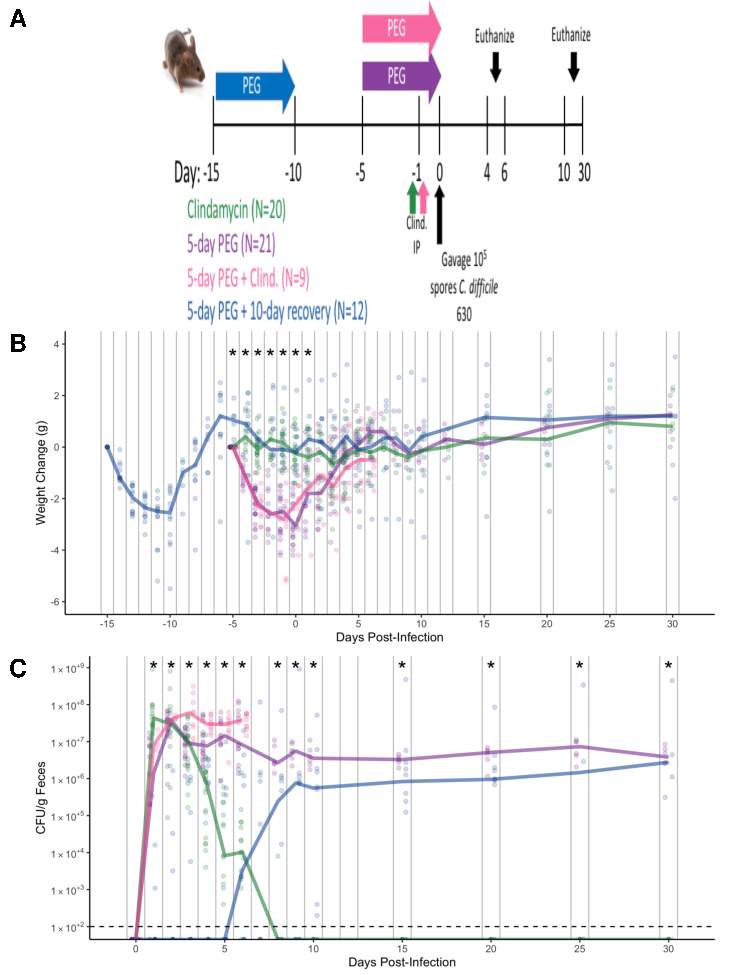
\includegraphics{figure_1.pdf}

\textbf{Figure 1. 5-day PEG treatment prolongs susceptibility and mice
become persistently colonized with \emph{C. difficile}.} A. Setup of the
experimental timeline for subset of experiments with 5-day PEG treated
mice. B. Weight change from baseline weight in groups after treatment
with PEG and/or clindamycin, followed by \emph{C. difficile} challenge.
C. \emph{C. difficile} CFU/gram stool measured over time (N =
4-\texttt{(insert\ variable\ name)} mice per timepoint) via serial
dilutions. The black line represents the limit of detection for the
first serial dilution. CFU quantification data was not available for
each mouse due to stool sampling difficulties (particularly the day the
mice came off of the PEG treatment) or early deaths. Lines represent the
median for each source and circles represent individual mouse samples.
Asterisks indicate timepoints where the weight change or CFU/g was
significantly different between groups by the Kruskal-Wallis test with
Benjamini-Hochberg correction for testing multiple timepoints. \newpage

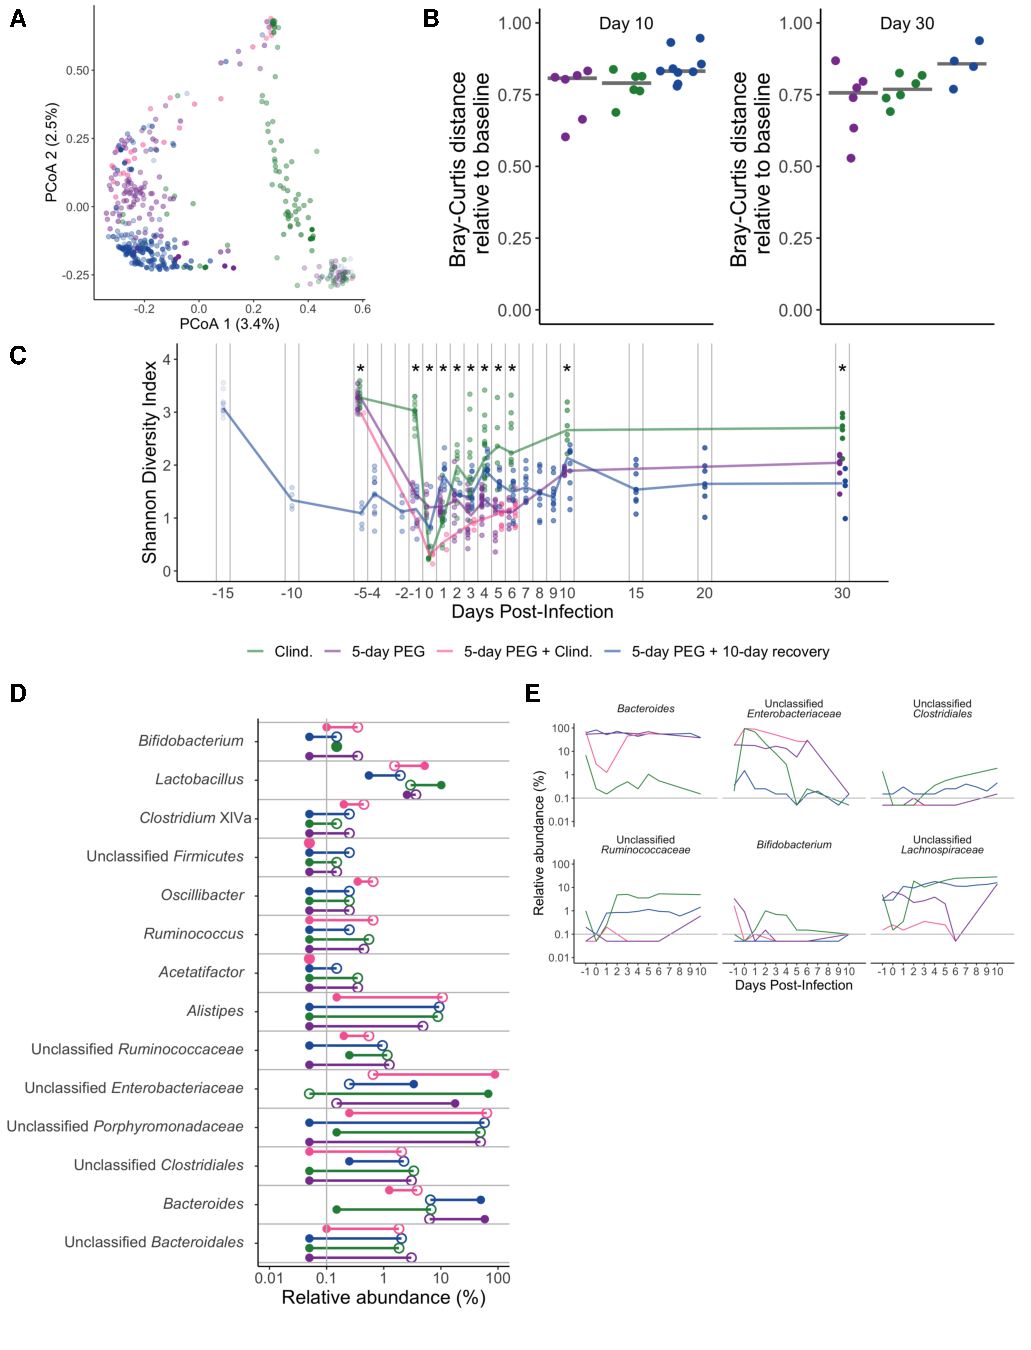
\includegraphics{figure_2.pdf} \textbf{Figure 2. 5-day PEG treatment
disrupts the stool microbiota for a longer amount of time compared to
clindamycin-treated mice.} A. \newpage

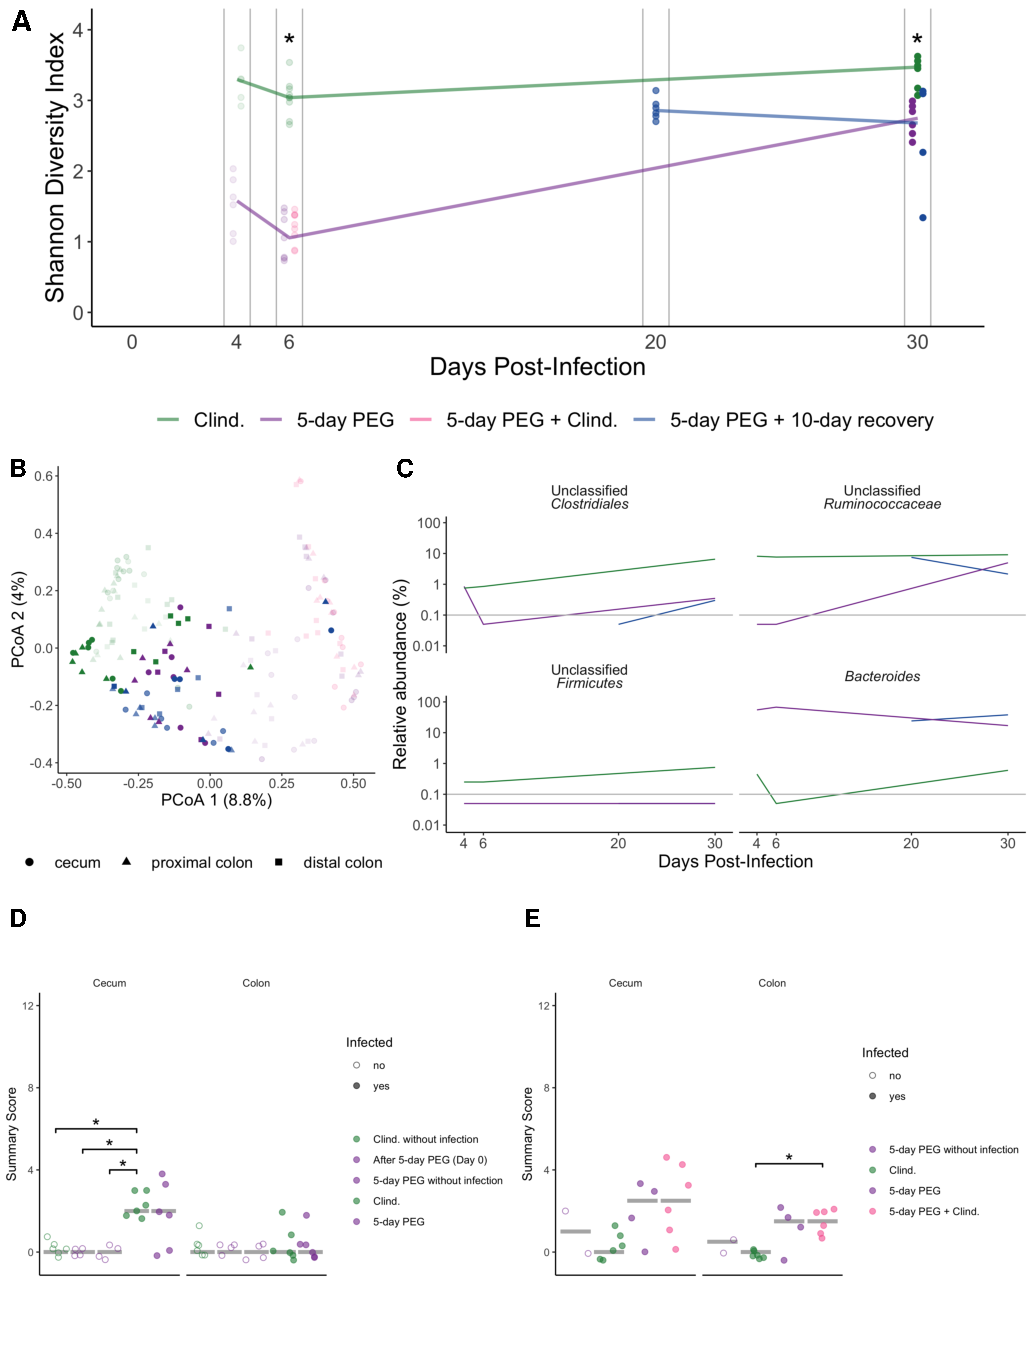
\includegraphics{figure_3.pdf} \textbf{Figure 3. 5-day PEG treatment
does not result in more severe CDIs, although mucosal microbiota is
altered.} A. \newpage

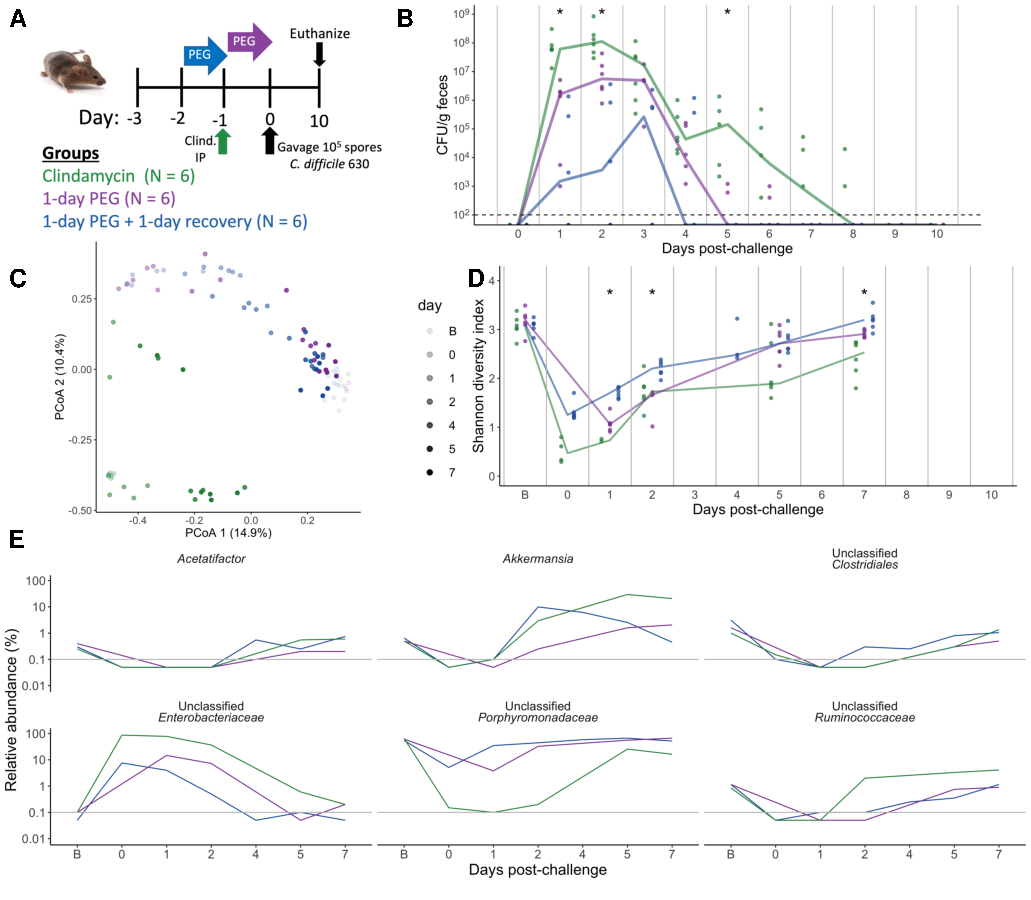
\includegraphics{figure_4.pdf} \textbf{Figure 4. 1-day PEG treatment
renders mice susceptible to transient \emph{C. difficile} colonization.}
A. Setup of the experimental timeline for the 1-day PEG treated subset
of mice. B. CFU/gram stool measured over time (N = 6 mice per timepoint)
via several dilutions. The black dotted line represents the limit of
detection for the first serial dilution. Asterisks indicate timepoints
where the CFU/gram was siginificantly different between groups using the
Kruskall-Wallis test with a Benjamini-Hochberg correction for multiple
timepoints. C. Principle Coordinate Analysis plot of the groups over
time with the alpha representating the same time scale as in panel D (P
= 1 R\textsuperscript{2} = 1). D. Shannon Diveristy Index of the groups
over time. Only days with samples from all groups are shown. Samples for
some mice were difficult to obtain due to the laxative treatment. The
alpha scale follows accordingly with the timeline. E. Line plots of
relative percent abundance of selected genera over time. Only days with
samples from all groups shown. The gray line represents the limit of
detection.

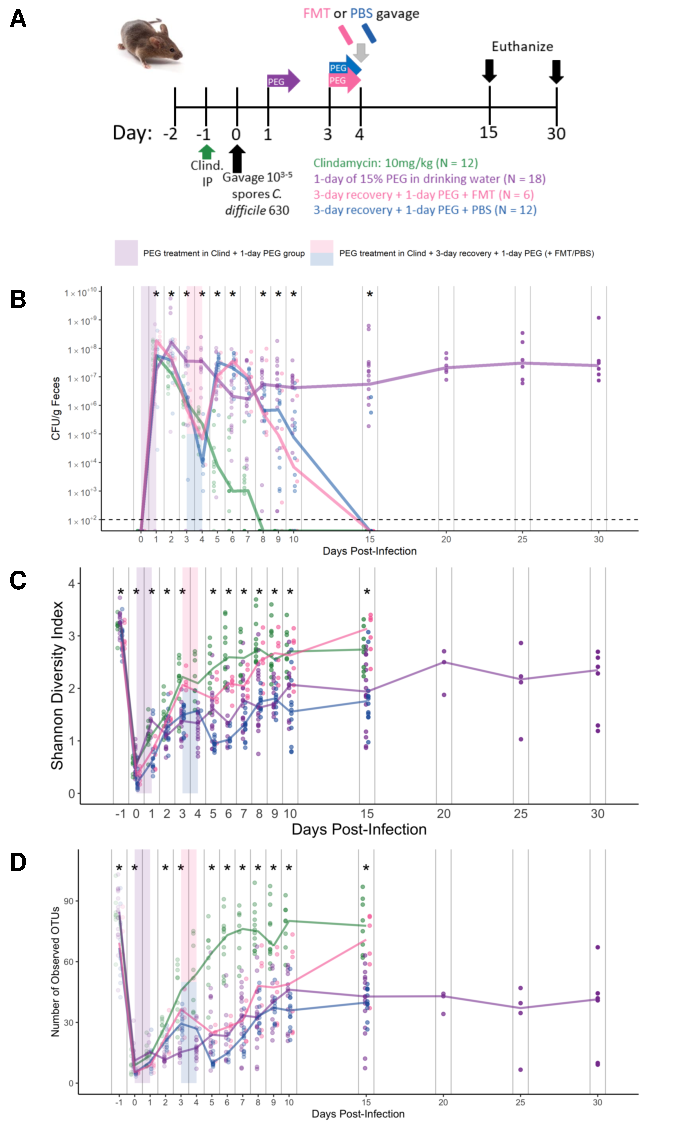
\includegraphics{figure_5.pdf} 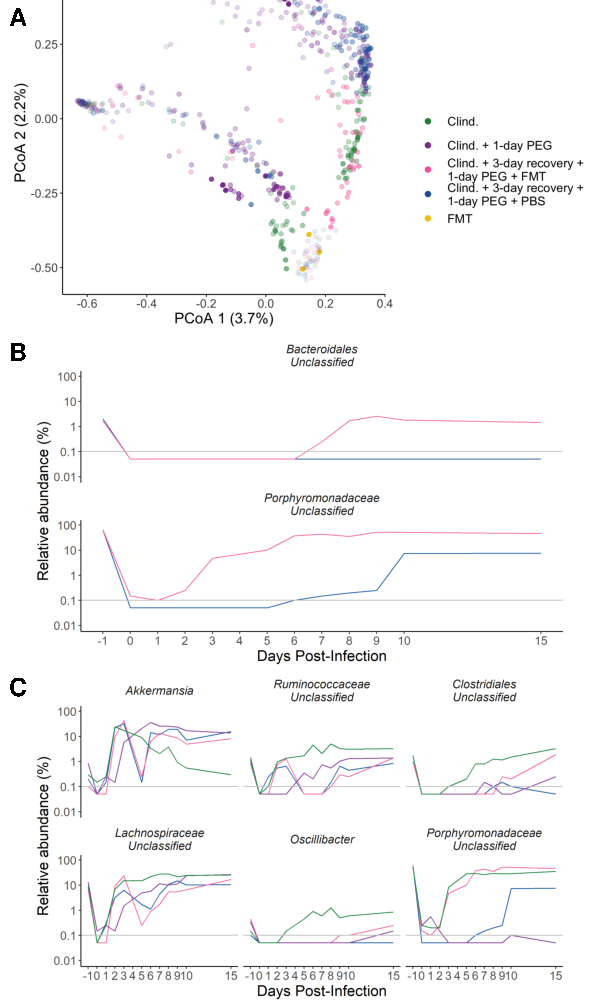
\includegraphics{figure_5_16S.pdf}
\textbf{Figure 5. 1-day PEG treatment post C. difficile challenge
prolongs colonization regardless of whether an FMT is also
administered.} A. \newpage

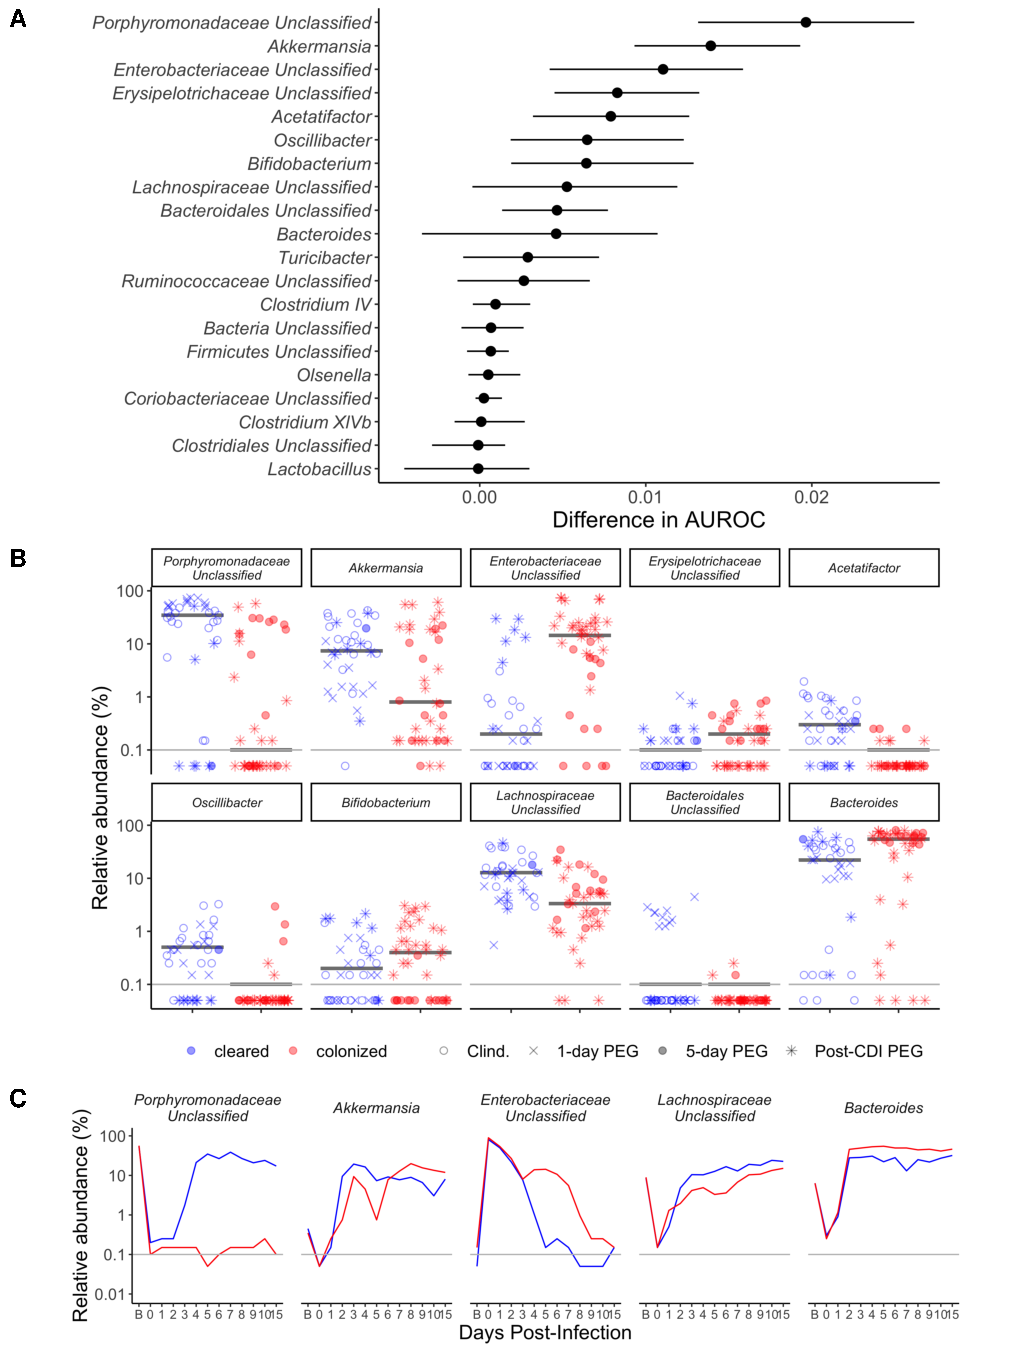
\includegraphics{figure_6.pdf} \textbf{Figure 6. Specific microbiota
features associated with prolonged \emph{C. difficile} colonization in
PEG treated mice.} A. \newpage

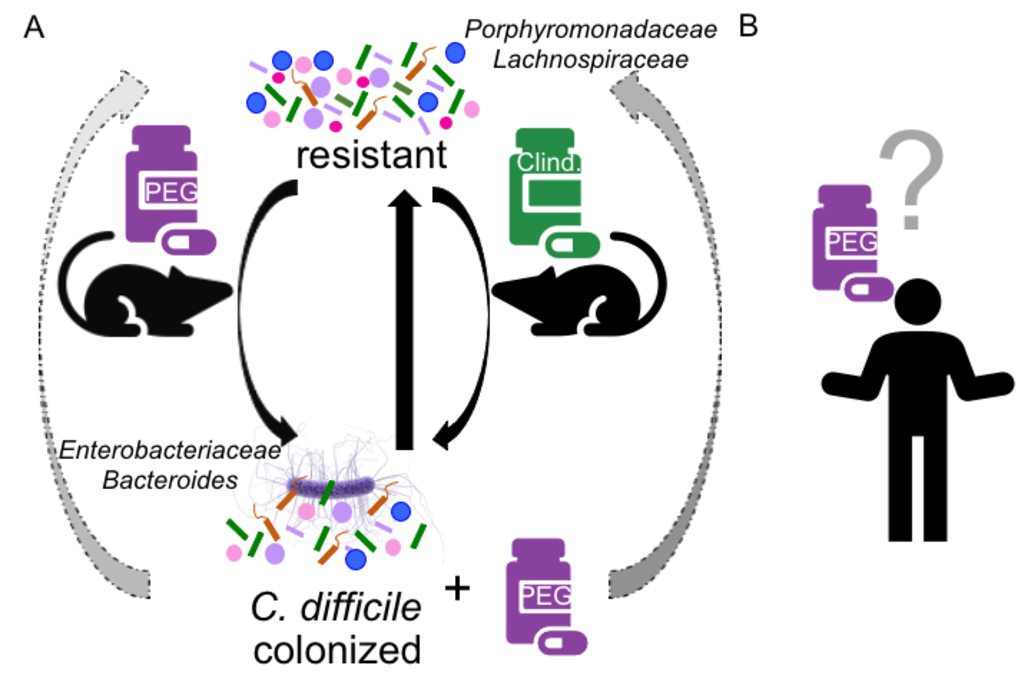
\includegraphics{figure_7.pdf} \textbf{Figure 7. Schematic summarizing
findings.} A. \newpage

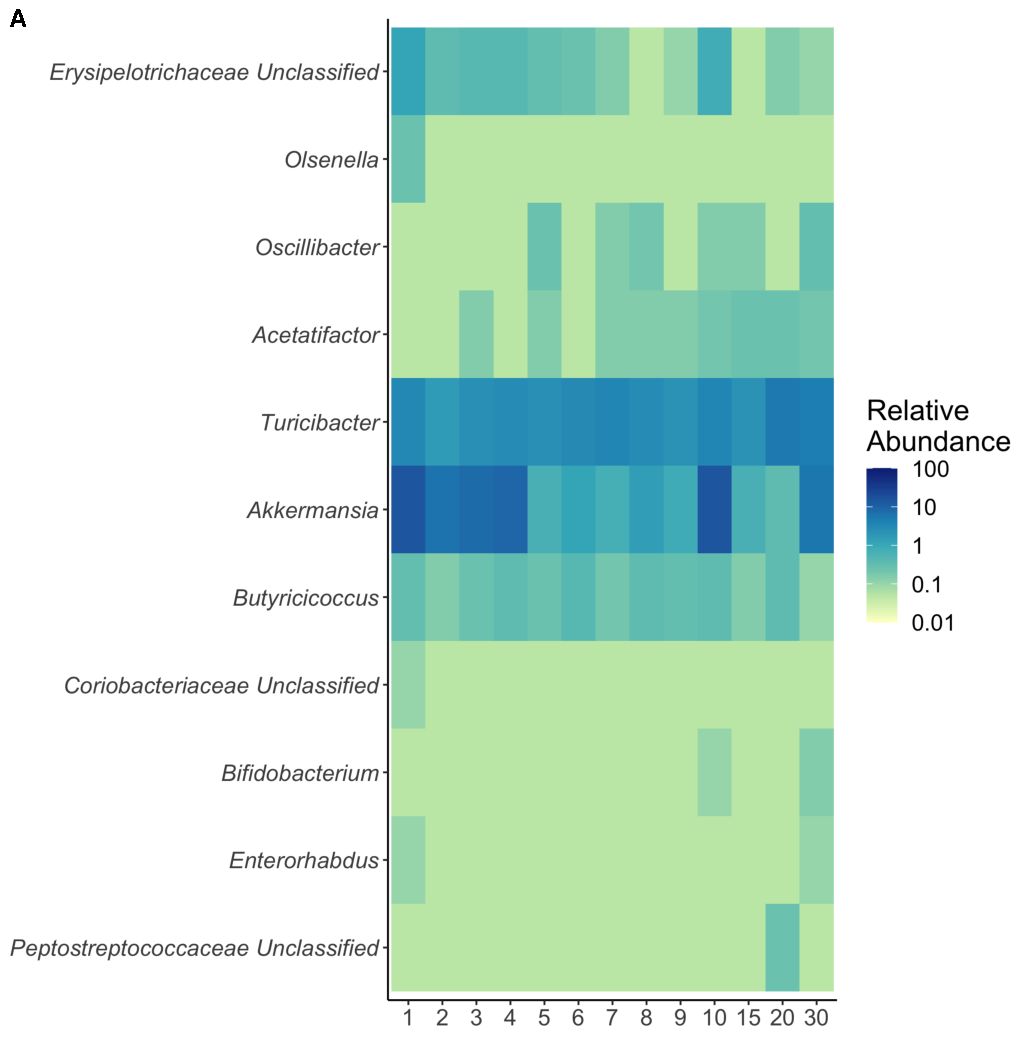
\includegraphics{figure_S1.pdf} \textbf{Figure S1. 5-day PEG treatment
plus 10-day recovery mice microbiota dynamics post-infection.} A.
\newpage

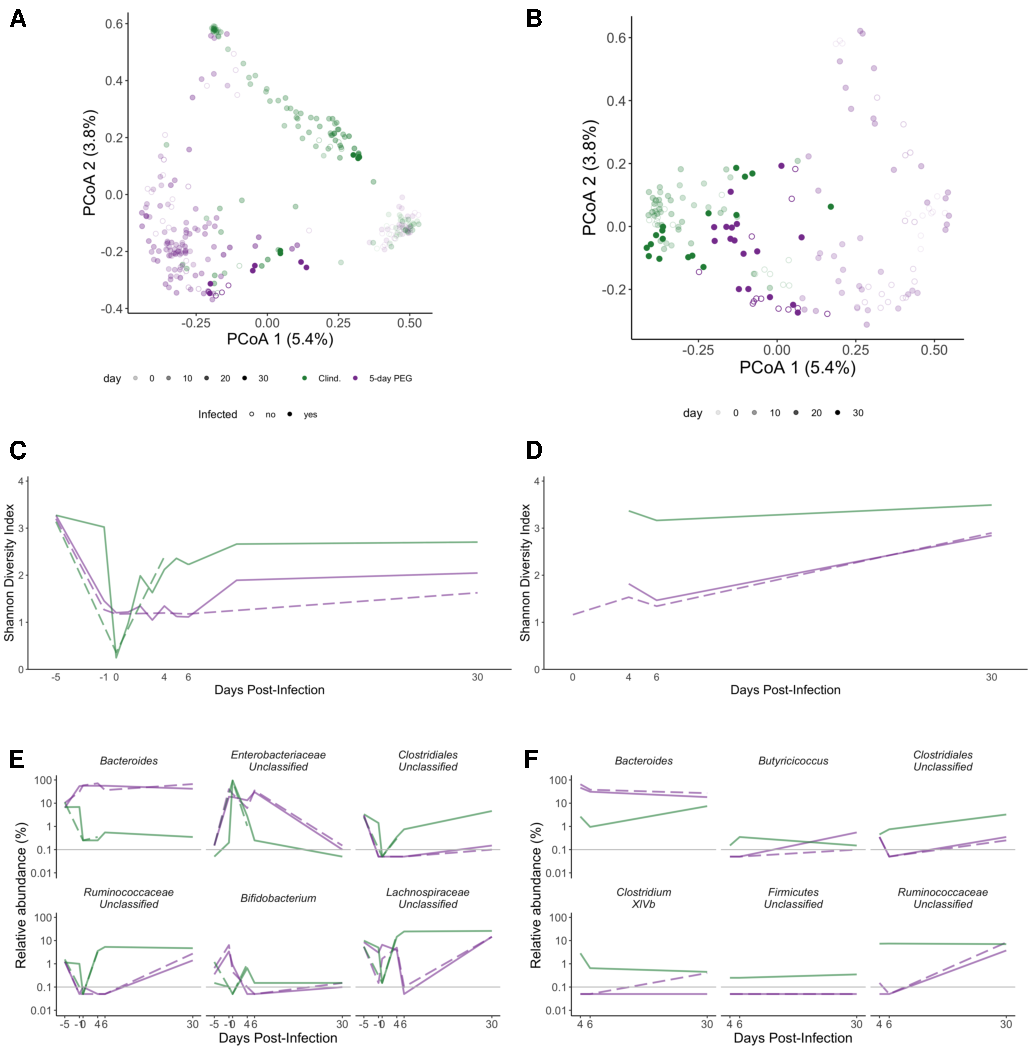
\includegraphics{figure_S2.pdf} \textbf{Figure S2. Specific OTUs
associated with clearance that are mostly absent in mice with prolonged
\emph{C. difficile} colonization. Ex. \emph{Muribaculum intestinale}.}
A. \newpage

\hypertarget{references}{%
\subsection{References}\label{references}}

\end{document}
